\chapter{Experiments and Results}

\section{Experimental Setup}

All experiments use Mind2Web \cite{deng2023mind2webgeneralistagentweb}, which is common available standard benchmark for element-level grounding. Dataset also support three splits: \texttt{test\_task} (1,339 samples, Tasks from the same website are seen during training), \texttt{test\_website} (1,019 samples,  Websites are not seen during training), and \texttt{test\_domain} (4,060 samples,  Entire domains are not seen during training). The full evaluation set is 6,418 samples. Training uses the Mind2Web train/eval splits (7775 train / 736 eval) released by the dataset authors. Fig \ref{fig:grounder_fine-tune} our initial training environment values.


\begin{figure}[!h]
    \centering    
    \begin{subfigure}[t]{0.48\linewidth}
        \centering
        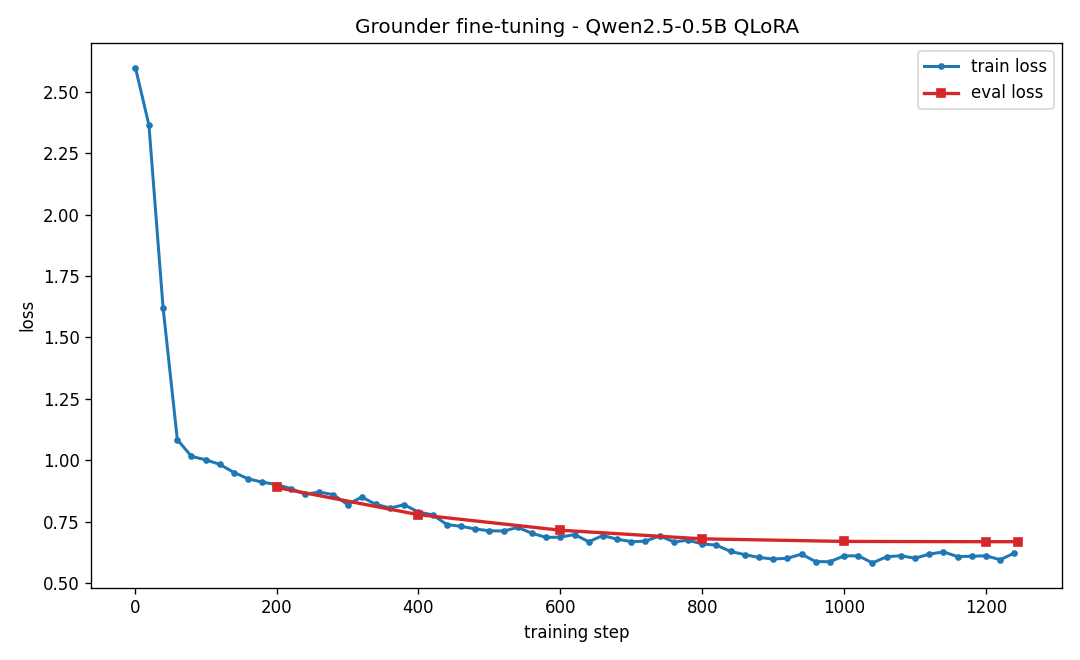
\includegraphics[width=\linewidth]{Charts/loss_curve_Qwen2.png}
        \caption{grounder fine-tuning Qwen2.5-0.5B model}
    \end{subfigure}
    \hfill
    \begin{subfigure}[t]{0.48\linewidth}
        \centering
        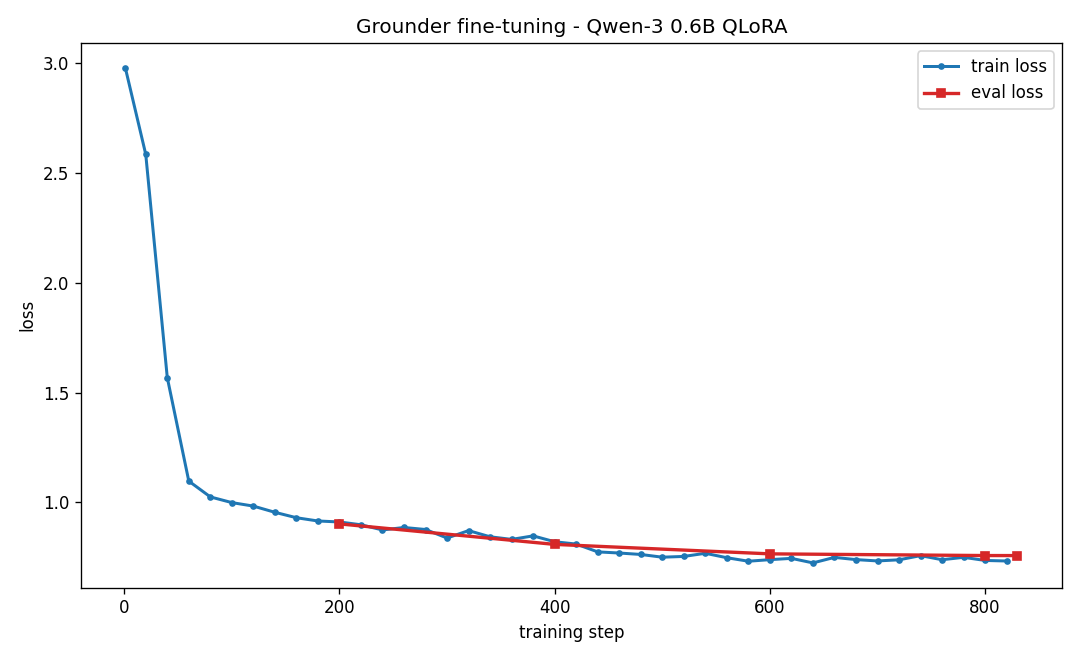
\includegraphics[width=\linewidth]{Charts/loss_curve_qwen3.png}
        \caption{grounder fine-tuning Qwen3-0.6B model}
    \end{subfigure}

    \caption{Traning loss curves}
    \label{fig:grounder_fine-tune}
\end{figure}

\textbf{Recall@20} measures whether the ground-truth element listed in the top-20 candidates returned after filter. \cite{deng2023mind2webgeneralistagentweb}. \textbf{Element Accuracy (EA)} is generated result by the Grounder matche the ground truth value \cite{zhang2025prune4web}.

Hardware used around all experiment is RTX 4050 GPU (6 GB VRAM) with CUDA for inference. All grounders are 4-bit QLoRA \cite{dettmers2023qlora} with rank \texttt{r=16}, \texttt{alpha=32}, effective batch size=16, max sequence length=1024, and seed value=42. In results chapter we compare Four types of implemented filter as \textbf{FULL} (Prune4Web's keyword-weighted scoring on all candidates, serving as the paper baseline), \textbf{DELTA\_KW} (a delta-aware keyword prefilter), \textbf{DELTA\_EMBED} (MiniLM cosine ranking only), and \textbf{DELTA\_HYBRID} (Hybrid approach of combining keyword and embedings filter: $\alpha \cdot \mathrm{keyword} + (1-\alpha) \cdot \mathrm{MiniLM}$ with $\alpha = 0.6$).


% \section{Token Reduction}

% We used Qwen's own BPE tokenizer rather than a character-length proxy, so that the numbers are directly comparable to what the LLM directly takes as input. The same 500-sample test\_domain from the Multimodel dataset was tokenised with the Qwen2.5-0.5B tokenizer and with the Qwen3-0.6B tokenizer. Table \ref{tab:tokenizer} reports the results.

% \begin{table}[h]
% \centering
% \small
% \begin{tabular}{l|r|r|r|r|r}
% \hline
% \textbf{Config} & \textbf{Recall@20} & \textbf{Char proxy} & \textbf{Qwen tokens} & \textbf{Char red.} & \textbf{Token red.} \\
% \hline
% FULL & 86.60\% & 1{,}383 & 429.6 & --- & --- \\
% DELTA\_KW & 85.20\% & 1{,}112 & 342.0 & 19.6\% & \textbf{20.4\%} \\
% DELTA\_EMBED & 86.00\% & 898 & 321.4 & 35.1\% & \textbf{25.2\%} \\
% \textbf{DELTA\_HYBRID} & \textbf{88.80\%} & 1{,}158 & 380.0 & 16.3\% & \textbf{11.5\%} \\
% \hline
% \end{tabular}
% \caption{Qwen tokenizer token-cost comparison across filter configurations on 500 test\_domain samples. The Qwen2.5 and Qwen3 tokenizers produced byte-for-byte identical counts, so the analysis applies to both grounders unchanged.}
% \label{tab:tokenizer}
% \end{table}

% The two tokenizers produced byte-for-byte identical token counts across all 500 samples, which confirms that Qwen3 inherits Qwen2.5's BPE merges without modification \cite{qwen25techreport2024}. The character-length proxy and actual Qwen tokens do not track linearly, because the DOM element summaries contain many special-looking tokens (tag names, attribute keys, separators) that the Qwen BPE merges into single tokens while the character proxy over-counts them. The Qwen token-reduction numbers are the ones that should be reported in cost estimates; they are roughly 30\% smaller than the character-proxy numbers but still clearly positive for every delta configuration.


\section{Filter-Stage Recall@20}

This sectioncontain Recall@20 details of the Filtering of DOM using implemented methadologies. This is important as it define wheather ground thuruth element is actually available in top N (where N=20) even after performing the filter. Based on this filtered element only Grounder will infer in pipeline for Actual Element. Table \ref{tab:recall} contain Recall@20 and token cost values for all four implementation configuration, across all three Mind2Web test splits (6{,}070 samples in total).

\begin{table}[!h]
\footnotesize
\centering
\begin{tabularx}{\textwidth}{X|X|X|X|X|X|c}
\hline
\textbf{Split} & \textbf{Config} & \textbf{Recall@20} & \textbf{Tokens} & \textbf{Lat. (ms)} & \textbf{$\Delta$ Recall} & \textbf{Tok. red.} \\
\hline
test\_task (1{,}257)     & FULL & 84.88\% & 1{,}432 & 9.60 & --- & --- \\
                         & $\Delta$\_KW & 84.57\% & 1{,}142 & 2.88 & -0.31 pp & 20.3\% \\
                         & $\Delta$\_EMBED & 82.26\% & 907 & 150.01 & -2.62 pp & 36.7\% \\
                         & \textbf{$\Delta$\_HYBRID} & \textbf{84.65\%} & \textbf{1{,}196} & \textbf{152.56} & \textbf{-0.23 pp} & \textbf{16.5\%} \\
\hline
test\_website (975)      & FULL & 88.62\% & 1{,}357 & 7.76 & --- & --- \\
                         & $\Delta$\_KW & 88.21\% & 1{,}059 & 2.31 & -0.41 pp & 22.0\% \\
                         & $\Delta$\_EMBED & 87.18\% & 845 & 142.55 & -1.44 pp & 37.8\% \\
                         & \textbf{$\Delta$\_HYBRID} & \textbf{88.51\%} & \textbf{1{,}117} & \textbf{144.70} & \textbf{-0.11 pp} & \textbf{17.7\%} \\
\hline
test\_domain (3{,}838)   & FULL & 87.23\% & 1{,}373 & 7.40 & --- & --- \\
                         & $\Delta$\_KW & 86.22\% & 1{,}085 & 2.02 & -1.01 pp & 21.0\% \\
                         & $\Delta$\_EMBED & 86.16\% & 883 & 122.07 & -1.07 pp & 35.7\% \\
                         & \textbf{$\Delta$\_HYBRID} & \textbf{88.43\%} & \textbf{1{,}142} & \textbf{122.77} & \textbf{+1.20 pp} & \textbf{16.9\%} \\
\hline
\end{tabularx}
\caption{DOM Delta A/B benchmark on all Mind2Web test splits (6{,}070 samples). DELTA\_HYBRID matches or improves Recall@20 while consistently reducing grounder input by 16-18\%.}
\label{tab:recall}
\end{table}

DELTA\_HYBRID scores 0.23~pp over the FULL baseline on test\_task and test\_website, and recall also improved by +1.20~pp on test\_domain. On unseen domains, experiment results show better results with cheaper inference cost (16 to 18\% token reduction) without much higher difference in Recall@20. Pure DELTA\_EMBED (embedding-based filter) loses 1 to 3 pp of recall across all splits, which is why the hybrid fusion (with $\alpha = 0.6$) is preferred over embeddings alone.


\section{Grounder Element Accuracy}

Core Sub-task success rate majorly dependce on the Grounded Element Accuracy value. Two local grounders (from Qwen series) are used, both finetuned with the identical QLoRA method on the same 6,626 Mind2Web examples, and we compare them against the 88.28\% test\_task number from the Prune4Web paper, which fine-tuned using Qwen2.5VL-3B-Instruct vision-language grounder \cite{zhang2025prune4web}.

\subsection{Qwen2.5-0.5B LoRA grounder}

Table \ref{tab:ea_qwen25} contains the Element Accuracy of the 0.5B local grounder on a 200-sample test\_domain slice, experimented with both the FULL and DELTA\_HYBRID candidate blocks.

\begin{table}[h]
\centering
\small
\begin{tabular}{l|r|r|r|r}
\hline
\textbf{Config} & \textbf{Recall@20} & \textbf{Element Accuracy} & \textbf{Char tokens} & \textbf{Token red.} \\
\hline
FULL & 90.50\% & \textbf{73.00\%} & 1{,}349 & --- \\
DELTA\_HYBRID & 89.50\% & 68.00\% & 1{,}153 & 14.5\% \\
\hline
\end{tabular}
\caption{Element Accuracy with the Qwen2.5-0.5B + LoRA grounder, on 200 test\_domain samples.}
\label{tab:ea_qwen25}
\end{table}

On the separate test\_task split (200 samples, same LoRA adapter), the Qwen2.5-0.5B grounder achieves 85.00\% EA, which is 3.28~\% lesser than Web4Prune's given 88.28\%, but Qwen2.5VL-3B-Instruct, which is a roughly 6x fewer parameters model and without the vision encoder.

\subsection{Qwen3-0.6B LoRA grounder}

Table \ref{tab:ea_qwen3} contains the same measurement with the newer Qwen3-0.6B base, fine-tuned with the same methodology.

\begin{table}[h]
\centering
\small
\begin{tabular}{l|r|r|r|r}
\hline
\textbf{Config} & \textbf{Recall@20} & \textbf{Element Accuracy} & \textbf{Char tokens} & \textbf{Token red.} \\
\hline
FULL & 90.50\% & \textbf{77.50\%} & 1{,}349 & --- \\
DELTA\_HYBRID & 89.50\% & 71.50\% & 1{,}153 & 14.5\% \\
\hline
\end{tabular}
\caption{Element Accuracy with the Qwen3-0.6B + LoRA grounder, on the same 200 test\_domain samples as Table \ref{tab:ea_qwen25}.}
\label{tab:ea_qwen3}
\end{table}

On test\_task (200 same samples), the Qwen3-0.6B grounder reaches 88.00\% EA, which matches the Prune4Web 88.28\% Qwen2.5VL-3B-Instruct number within a sub-sample rounding margin.

\subsection{Comparison against Prune4Web Qwen2.5VL-3B grounder}

Table \ref{tab:ea_sidebyside} three grounders comparison together.

\begin{table}[!h]
\small
\centering
\begin{tabularx}{\textwidth}{X|X|X|X|X}
\hline
\textbf{Eval (test\_domain, 200)} & \textbf{Qwen2.5VL-3B (Prune4Web)} & \textbf{Qwen2.5-0.5B} & \textbf{Qwen3-0.6B} & \textbf{Qwen3 - Qwen2.5} \\
\hline
test\_task EA & 88.28\% & 85.00\% & 88.00\% & +3.00 pp \\
DOM-Delta FULL EA & --- & 73.00\% & 77.50\% & +4.50 pp \\
DOM-Delta DELTA\_HYBRID EA & --- & 68.00\% & 71.50\% & +3.50 pp \\
\hline
\end{tabularx}
\caption{Side-by-side: the Prune4Web paper's fine-tuned Qwen2.5VL-3B-Instruct reference \cite{zhang2025prune4web} vs the two local QLoRA grounders. The Qwen3-0.6B LoRA matches the paper's 3B vision-language grounder on Mind2Web test\_task at roughly 5x fewer parameters and without a vision encoder.}
\label{tab:ea_sidebyside}
\end{table}

\begin{figure}[!h]
    \centering    
    \begin{subfigure}[t]{0.48\linewidth}
        \centering
        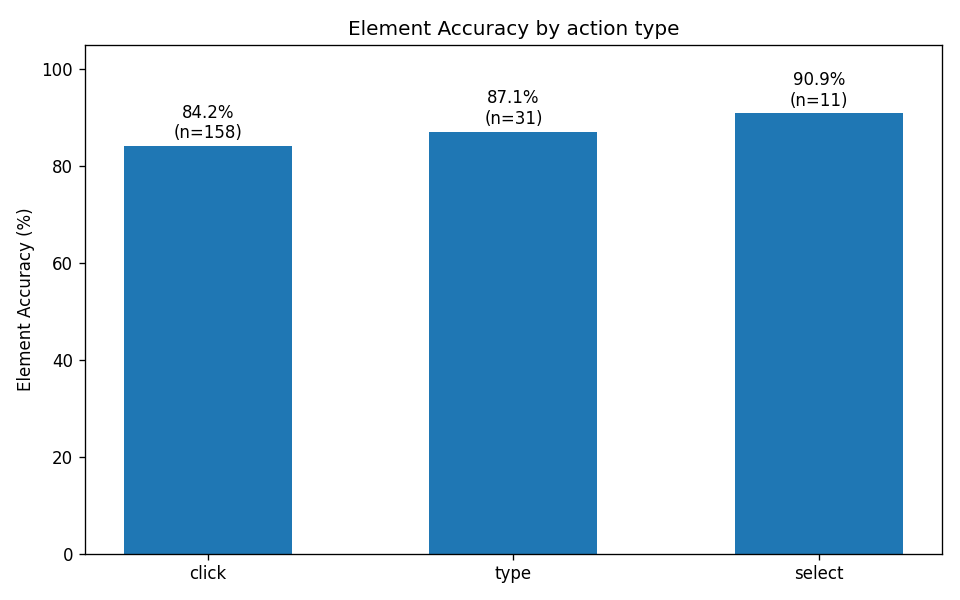
\includegraphics[width=\linewidth]{Charts/eval_by_action.png}
        \caption{EA with Qwen2.5-0.5B model}
    \end{subfigure}
    \hfill
    \begin{subfigure}[t]{0.48\linewidth}
        \centering
        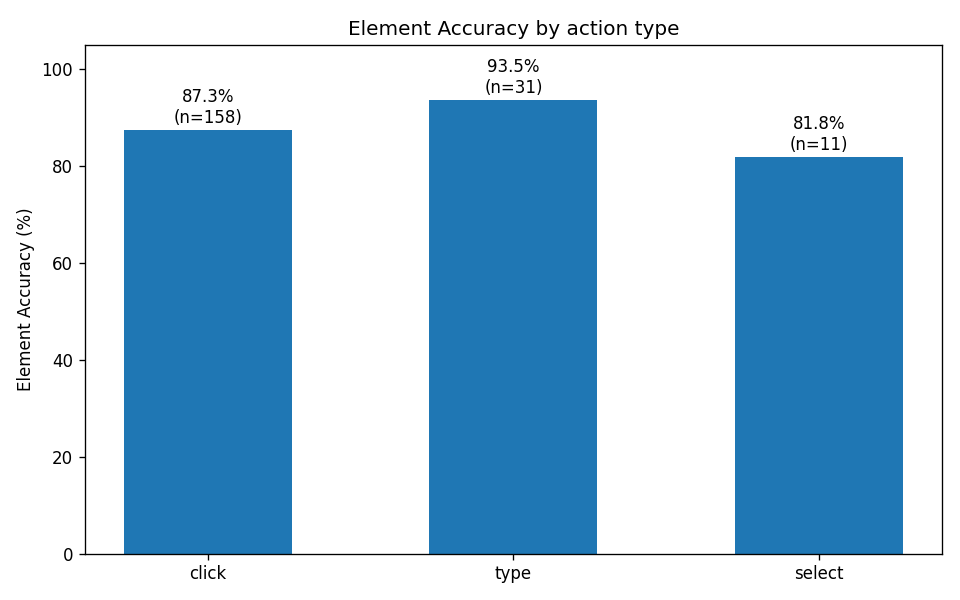
\includegraphics[width=\linewidth]{Charts/eval_by_action_3.0.png}
        \caption{EA with Qwen3-0.6B model}
    \end{subfigure}

    \caption{Action-wise element accuracycy}
    \label{fig:element_acuracy_comparision}
\end{figure}

Fig \ref{fig:element_acuracy_comparision} contain side by side action wise Element Acurassy between Qwen2.5 and Qwen3 model. Scaling the grounder from 0.5B to 0.6B with the recent version improves EA by 3 to 4.5~\% across all configurations with the filter side held exactly equal, so the gain clearly comes from the LLM and not from the filter. The DELTA\_HYBRID vs FULL gap of roughly 6~pp EA is stable across both grounders, even though their Recall@20 differs by only 1~pp. With the 200-sample slice giving a $\pm$6~\% 95\% confidence interval per cell, the reproducibility of this gap across two different grounder sizes argues that it is a genuine downstream sensitivity to candidate ordering rather than random noise. The recommended next step to close it is candidate-ordering normalisation (re-sorting the top-20 by structural UID or DOM position before building the grounder prompt).


% \section{Training Time and Inference Latency}

% Table \ref{tab:training} summarises the training cost of the two local grounders together with the Prune4Web paper's fine-tuned Qwen2.5VL-3B-Instruct \cite{zhang2025prune4web} as a reference. Both local grounders were trained on the same 6{,}626 Mind2Web examples with identical QLoRA hyperparameters.

% \begin{table}[h]
% \centering
% \small
% \begin{tabular}{l|r|r|r|r}
% \hline
% \textbf{Grounder} & \textbf{Params} & \textbf{Epochs} & \textbf{Train time} & \textbf{Final eval loss} \\
% \hline
% Qwen2.5VL-3B-Instruct (Prune4Web, fine-tuned) & $\sim$3B & --- & --- & --- \\
% Qwen2.5-0.5B + LoRA & 0.5B & 3 & 609 min & 0.668 \\
% \textbf{Qwen3-0.6B + LoRA} & \textbf{0.6B} & \textbf{2} & \textbf{325 min} & \textbf{0.758} \\
% \hline
% \end{tabular}
% \caption{Training cost of the two local grounders. Despite being 20\% larger, Qwen3-0.6B trained in 47\% less wall-clock time than Qwen2.5-0.5B, because we used 2 epochs instead of 3 and because Qwen3 converged faster per step.}
% \label{tab:training}
% \end{table}

% Qwen3-0.6B trained in roughly half the wall-clock time of Qwen2.5-0.5B, even though it is the larger model, because the loss curve for Qwen2.5 had largely plateaued by epoch 2 and the third epoch was added out of caution rather than necessity. Qwen3's slightly higher eval loss at 2 epochs (0.758 vs 0.668 for Qwen2.5 at 3 epochs) does \textit{not} reflect worse grounding performance; as Table \ref{tab:ea_sidebyside} shows, Qwen3's Element Accuracy is 3 to 4.5~pp \textit{higher}. The lower eval loss on Qwen2.5 looks more like overfitting to the JSON output format than actual improvement in grounding.

% On inference latency, Qwen2.5-0.5B is roughly 5~s per sample on an RTX 4050 while Qwen3-0.6B is roughly 20~s per sample. The difference is not due to the parameter count but to Qwen3's chat template, which still emits an empty \texttt{<think>\textbackslash n\textbackslash n</think>} block even when \texttt{enable\_thinking=False} is set. Those tokens must still be decoded before the JSON payload starts, which quadruples the decoding budget. For batch evaluation this is acceptable; for a live web-agent loop the lower-latency Qwen2.5 backend remains the cheaper choice, or alternatively the \texttt{<think>} block can be stripped at the tokenizer level.


\section{Latency Breakdown of DELTA\_HYBRID}

DELTA\_HYBRID is the recommended filter configuration, Thus we instrument its per-step cost on 200 test\_domain samples.

\begin{table}[h]
\centering
\small
\begin{tabular}{l|r|r}
\hline
\textbf{Stage} & \textbf{Time (ms)} & \textbf{\% of total} \\
\hline
Keyword scoring & 1.19 & 0.5\% \\
MiniLM encoding + score fusion & 222.08 & 99.5\% \\
\hline
\textbf{Total (per step)} & \textbf{223.29} & \textbf{100\%} \\
\hline
\end{tabular}
\caption{Per-step latency breakdown of DELTA\_HYBRID on 200 test\_domain samples (MiniLM on CUDA).}
\label{tab:latency}
\end{table}

\begin{figure}[!h]
    \centering
    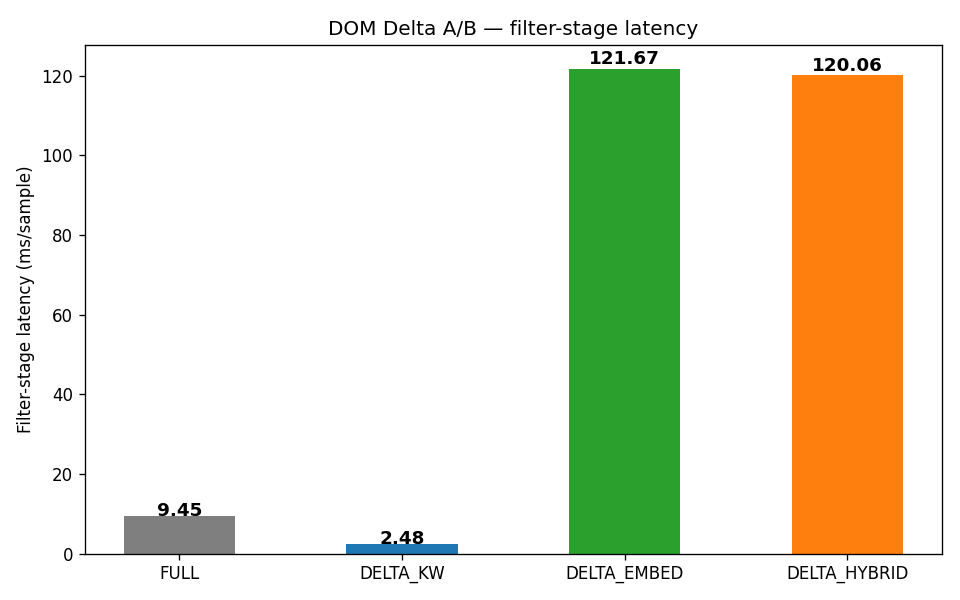
\includegraphics[width=0.5\linewidth]{Charts/latency.png}
    \caption{DOM Delta latency comparison between all type of configuration}
    \label{fig:latency}
\end{figure}

Fig \ref{fig:latency} contain the DOM Delta latency comparison accross all types of configuration. Almost all of the per-step cost is MiniLM inference on the candidate element summaries. At 120.06~ms, the filter adds very small latency to a web agent's typical 2 to 5~s per-step budget (network + screenshot + LLM call). Further speedups would require either a smaller encoder (for example MiniLM-L3) which may can reduce performance or caching embeddings of elements that are stable across steps (which the DOM Delta layer already identifies).


\section{Privacy and HITL}

Due to the lack of required dataset values availability, Privacy Hub + HITL just tested on very small live web sessions and does not have large-scale benchmark results. Mind2Web does not provide an annotated test for PII-annotation, nor are any HITL trigger tasks or subtasks available to compare with the ground truth value. As an experiment of PolicyHub's 24 risk keywords are defined with threshold value as 72\%, Where HITL successfully triggered on actions that involved password fields, CAPTCHA prompts, and payment-submit buttons pauses further pipeline for further human inputs. The PrivacyPipeline's regex-based PII detector was observed to mask email addresses, phone numbers, and date-of-birth patterns in element \texttt{value} and \texttt{placeholder} attributes before they reached the grounder prompt. A small number of around 14 samples online where 7 was required to trigger and 7 was not required to trigger HITL, as result of privacy hum 7 which not required trigger has not been triggered HITL, and 7 which was required trigger out of 1 falsely not triggered HITL, and 6 triggered HITL properly. Figure \ref{fig:HitlPrivacy} represent that heatmap of HITL trigger.

\begin{figure}[!h]
    \centering
    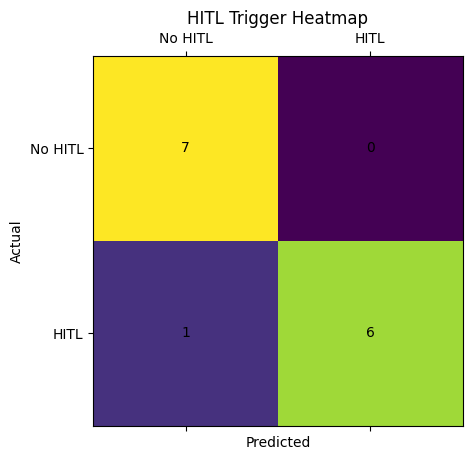
\includegraphics[width=0.5\linewidth]{HITL_Result.png}
    \caption{HITL triggers with perfect precision and with having 0.86 recall, where 1 actually should trigger HITL is not triggered.}
    \label{fig:HitlPrivacy}
\end{figure}


